%% System architecture of SafeStream-Redactor. Compiled to fig_architecture.pdf
%% (pdflatex fig_architecture.tex); main.tex includes the PDF.
\documentclass[border=4pt]{standalone}
\usepackage{tikz}
\usetikzlibrary{arrows.meta,positioning,fit,backgrounds,calc}
\usepackage[scaled=0.92]{helvet}
\renewcommand{\familydefault}{\sfdefault}

\definecolor{eng}{HTML}{2A78D6}
\definecolor{det}{HTML}{1BAF7A}
\definecolor{opt}{HTML}{8A8A8A}
\definecolor{out}{HTML}{EB6834}

\begin{document}
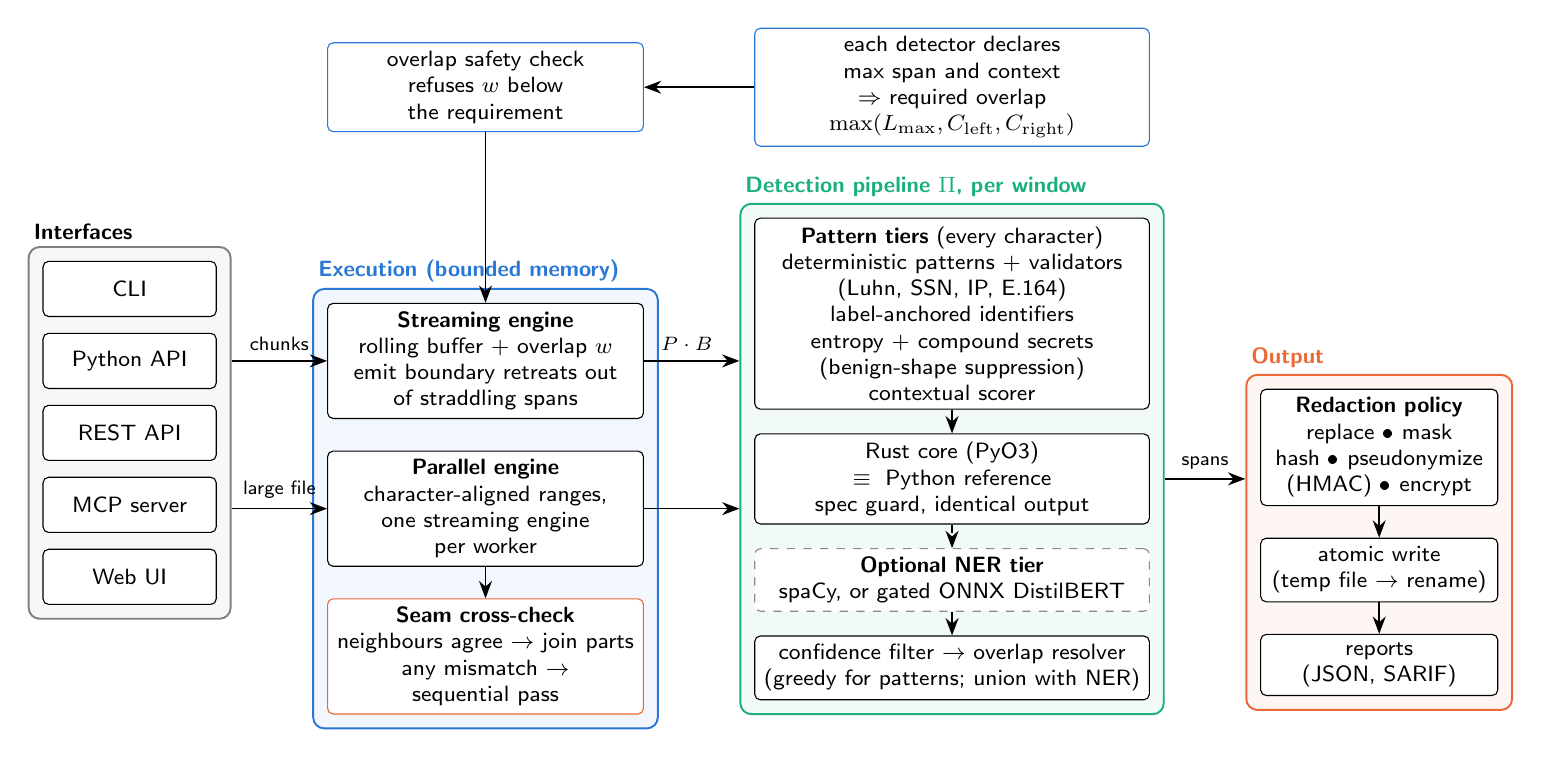
\begin{tikzpicture}[
  font=\footnotesize,
  node distance=4mm and 6mm,
  box/.style={draw, rounded corners=2pt, align=center, inner sep=3pt, minimum height=7mm, fill=white},
  grp/.style={draw, rounded corners=4pt, inner sep=5pt, line width=0.7pt},
  lbl/.style={font=\footnotesize\bfseries, anchor=south west, inner sep=2pt},
  arr/.style={-{Stealth[length=2.2mm]}, line width=0.6pt},
  darr/.style={-{Stealth[length=2.2mm]}, line width=0.6pt, dashed},
]

% ---------------- interfaces ----------------
\node[box, minimum width=22mm] (cli) {CLI};
\node[box, minimum width=22mm, below=2mm of cli] (py) {Python API};
\node[box, minimum width=22mm, below=2mm of py] (rest) {REST API};
\node[box, minimum width=22mm, below=2mm of rest] (mcp) {MCP server};
\node[box, minimum width=22mm, below=2mm of mcp] (ui) {Web UI};
\begin{scope}[on background layer]
\node[grp, draw=black!50, fill=black!3, fit=(cli)(ui)] (gin) {};
\end{scope}
\node[lbl] at (gin.north west) {Interfaces};

% ---------------- engines ----------------
\node[box, right=14mm of py, minimum width=40mm, text width=38mm] (stream)
  {\textbf{Streaming engine}\\ rolling buffer + overlap $w$\\ emit boundary retreats out\\ of straddling spans};
\node[box, below=4mm of stream, minimum width=40mm, text width=38mm] (par)
  {\textbf{Parallel engine}\\ character-aligned ranges,\\ one streaming engine\\ per worker};
\node[box, below=4mm of par, minimum width=40mm, text width=38mm, draw=out] (seam)
  {\textbf{Seam cross-check}\\ neighbours agree $\rightarrow$ join parts\\ any mismatch $\rightarrow$ sequential pass};
\begin{scope}[on background layer]
\node[grp, draw=eng, fill=eng!6, fit=(stream)(seam)] (geng) {};
\end{scope}
\node[lbl, text=eng] at (geng.north west) {Execution (bounded memory)};

% ---------------- detection ----------------
\node[box, right=14mm of stream, minimum width=50mm, text width=48mm, yshift=6mm] (t0)
  {\textbf{Pattern tiers} (every character)\\
   deterministic patterns + validators\\ (Luhn, SSN, IP, E.164)\\
   label-anchored identifiers\\
   entropy + compound secrets\\ (benign-shape suppression)\\
   contextual scorer};
\node[box, below=3mm of t0, minimum width=50mm, text width=48mm] (backend)
  {Rust core (PyO3) \;$\equiv$\; Python reference\\ spec guard, identical output};
\node[box, below=3mm of backend, minimum width=50mm, text width=48mm, draw=opt, dashed] (ner)
  {\textbf{Optional NER tier}\\ spaCy, or gated ONNX DistilBERT};
\node[box, below=3mm of ner, minimum width=50mm, text width=48mm] (res)
  {confidence filter $\rightarrow$ overlap resolver\\ (greedy for patterns; union with NER)};
\begin{scope}[on background layer]
\node[grp, draw=det, fill=det!6, fit=(t0)(res)] (gdet) {};
\end{scope}
\node[lbl, text=det] at (gdet.north west) {Detection pipeline $\Pi$, per window};

% ---------------- output ----------------
\node[box, right=14mm of backend, minimum width=30mm, text width=28mm, yshift=4mm] (pol)
  {\textbf{Redaction policy}\\ replace \textbullet\ mask\\ hash \textbullet\ pseudonymize\\ (HMAC) \textbullet\ encrypt};
\node[box, below=4mm of pol, minimum width=30mm, text width=28mm] (atomic)
  {atomic write\\ (temp file $\rightarrow$ rename)};
\node[box, below=4mm of atomic, minimum width=30mm, text width=28mm] (rep)
  {reports\\ (JSON, SARIF)};
\begin{scope}[on background layer]
\node[grp, draw=out, fill=out!6, fit=(pol)(rep)] (gout) {};
\end{scope}
\node[lbl, text=out] at (gout.north west) {Output};

% ---------------- safety check (top band) ----------------
\node[box, draw=eng, above=9mm of t0, minimum width=50mm, text width=48mm] (req)
  {each detector declares max span and context\\ $\Rightarrow$ required overlap $\max(L_{\max}, C_{\mathrm{left}}, C_{\mathrm{right}})$};
\node[box, draw=eng, left=14mm of req, minimum width=40mm, text width=38mm] (guard)
  {overlap safety check\\ refuses $w$ below the requirement};

% ---------------- arrows ----------------
\draw[arr] (gin.east |- stream) -- node[above, font=\scriptsize]{chunks} (stream.west);
\draw[arr] (gin.east |- par) -- node[above, font=\scriptsize]{large file} (par.west);
\draw[arr] (stream.east) -- node[above, font=\scriptsize, pos=0.45]{$P\cdot B$} (gdet.west |- stream);
\draw[arr] (par.east) -- (gdet.west |- par);
\draw[arr] (par) -- (seam);
\draw[arr] (req) -- (guard);
\draw[arr] (guard) -- (stream.north);
\draw[arr] (gdet.east |- backend) -- node[above, font=\scriptsize]{spans} (gout.west |- backend);
\draw[arr] (pol) -- (atomic);
\draw[arr] (atomic) -- (rep);
\draw[arr] (t0.south) -- (backend.north);
\draw[darr] (backend) -- (ner);
\draw[arr] (ner) -- (res);
\end{tikzpicture}
\end{document}
